%\documentclass[prb,twocolumn,showpacs,aps,floats,floatfix,superscriptaddress]{revtex4}
%\documentclass[prb,showpacs,aps,floats,floatfix,superscriptaddress]{revtex4}
%\documentclass{article}
%\usepackage{epsfig,amsmath,amssymb,array,dcolumn,subfigure,rotating}

\documentclass[onecolumn,letterpaper,amsmath,amssymb,floatfix,aps,superscriptaddress]{revtex4}
%\documentclass[a4paper]{article}
\usepackage{graphicx}% Include figure files
\usepackage{dcolumn}% Align table columns on decimal point
\usepackage{bm}% bold math
\usepackage{epsfig,color}
\usepackage{wrapfig}


\usepackage{epsfig}

\def\ul#1#2{\textstyle{\frac#1#2}}
\def\rot{\operatorname{rot}}
\def\diver{\operatorname{div}}
\def\bnabla{\mbox{\boldmath $\nabla $}}
\def\bepsilon{\mbox{\boldmath $\epsilon $}}

\begin{document}

\title{\bf Tables of Hamaker coefficents results- For comparison of published, Gecko
Hamaker, and Python values for perpendicular cylinders in water}

\author{April 2, 2014}
    
\begin{abstract}
Rajter's results were calculated using a water LDS with large peak at n=0, Int.
J. Mat. Res 101 (2010).  Gecko Hamaker and Python results use Dan's water
spectrum.
%Dan sent some data, I made A's. He generated A's from GH. I plotted both results for comparison. They should agree. They don't.
\end{abstract}

\maketitle        
%
%\section{Imaginary part of the dielectric response function and Anisotropy metric}
%
%The dielectric response functions are evaluated at imaginary frequencies, 
%thus $\epsilon_{\parallel,\perp} = \epsilon_{\parallel,\perp}(i \omega)$. $\epsilon_{\parallel,\perp}(i \omega)$ is referred to as the London - van der Waals 
%transform of the response function $\epsilon_{\parallel,\perp}(\omega)$ and is given by the Kramers - Kronig relations. It is strictly a real, monotonically 
%decaying function of $\omega$. 
%%%%%%%%%EPS2 and Aiz%%%%%%%%%%%%%%%%%%%%%%%%%%%%%%%%%%%%%%%%%%%%%%%%
\begin{figure*}[t!]
\begin{center}
\begin{minipage}[b]{0.40\textwidth}
\begin{center}
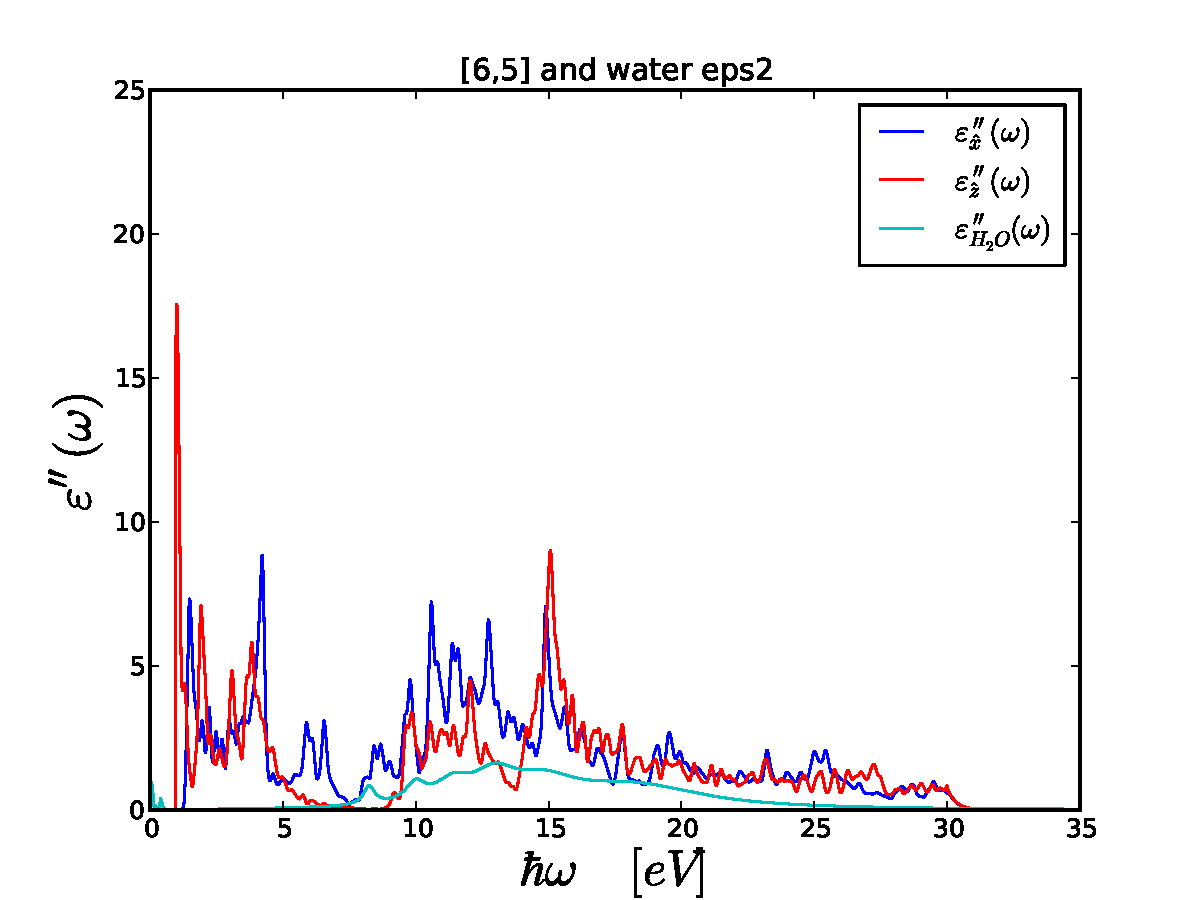
\includegraphics[width=1.0\textwidth]{prop_plots/65w65_eps2.pdf} (a)
\end{center}
\end{minipage}
\hskip 43pt
\begin{minipage}[b]{0.40\textwidth}
\begin{center}
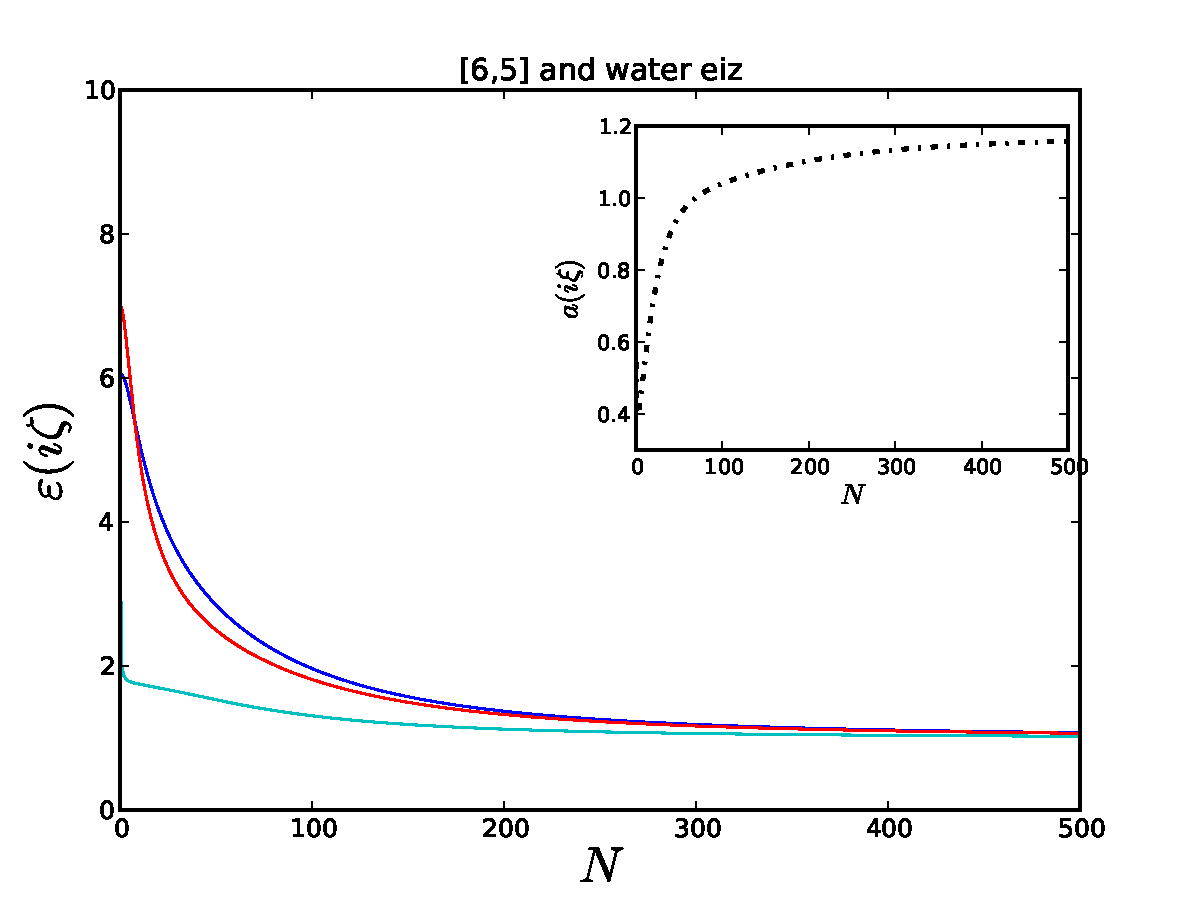
\includegraphics[width=1.0\textwidth]{prop_plots/65w65_eiz.pdf} (b)
\end{center}
\end{minipage}
\caption{Full result using Eqs.\ref{pars-31},\ref{pars-31-g} (a) Anisotropic response functions for CG-10 DNA and water. The DNA response functions in the x and y directions were used as perpendicular and parallel inputs, respectively.  CG-10 and water eps2 data was provided by Dan Dryden. CG-10 data scales Wai-Yim's calculations by 4.94 and is assumed to include Na (more info in Dan Dryden email sent to us on Nov. 8, 2013).  Water data was built from lorentz oscillators R.H.French,J.Amer.Ceram Soc.,83,9,2117-46(2000), H.D.Ackler, et al,J.Coll.Interface Sci.179,46.
(b) Anisotropy metric $a_{1,2}(i\zeta_n)$ using Eq.\ref{eq:adef}, compares the anisotropy of the  cylinders (DNA) to their intervening material, water for the terms contruting to the Matsubara sum.}
\label{eiz65}
\end{center}
\end{figure*} 

%%%%%%%%%EPS2 and Aiz%%%%%%%%%%%%%%%%%%%%%%%%%%%%%%%%%%%%%%%%%%%%%%%%
\begin{figure*}[t!]
\begin{center}
\begin{minipage}[b]{0.40\textwidth}
\begin{center}
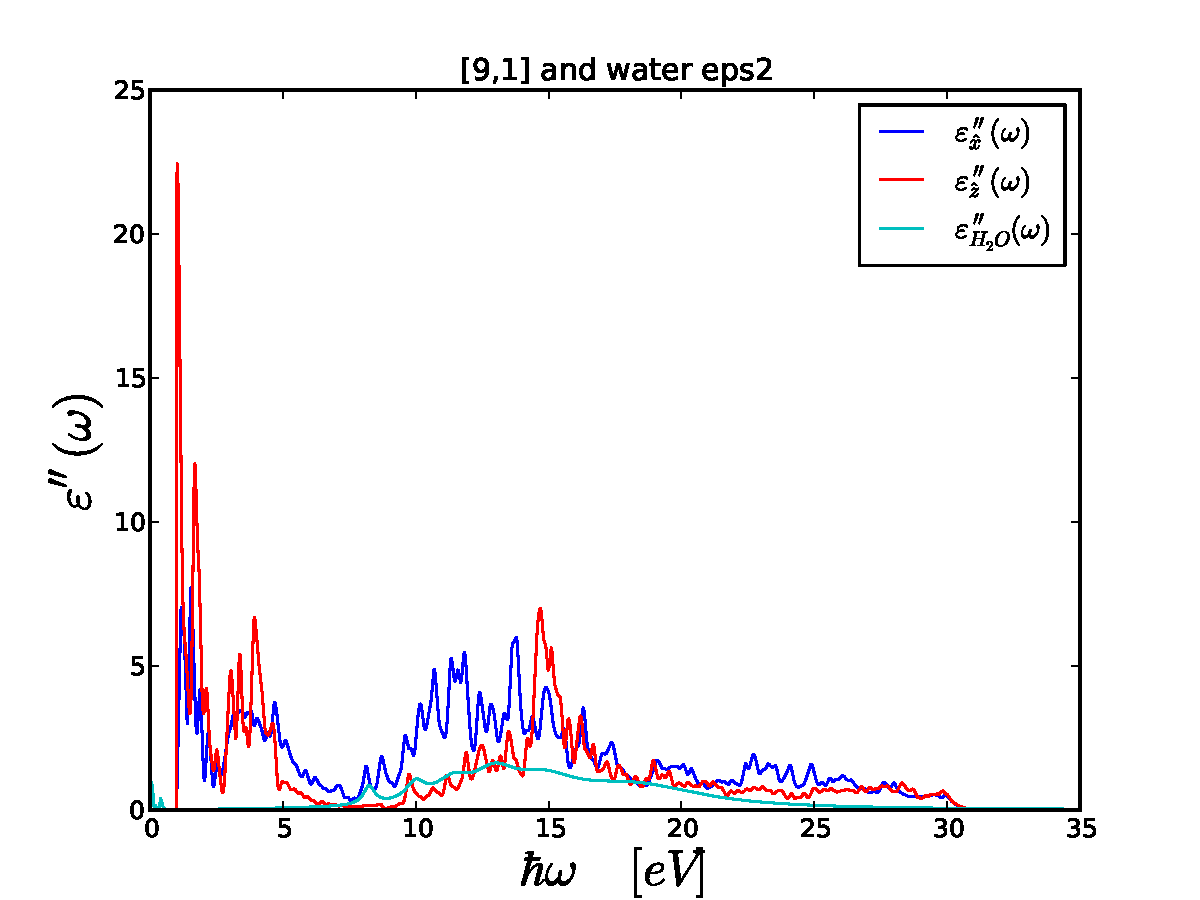
\includegraphics[width=1.0\textwidth]{prop_plots/91w91_eps2.pdf} (a)
\end{center}
\end{minipage}
\hskip 43pt
\begin{minipage}[b]{0.40\textwidth}
\begin{center}
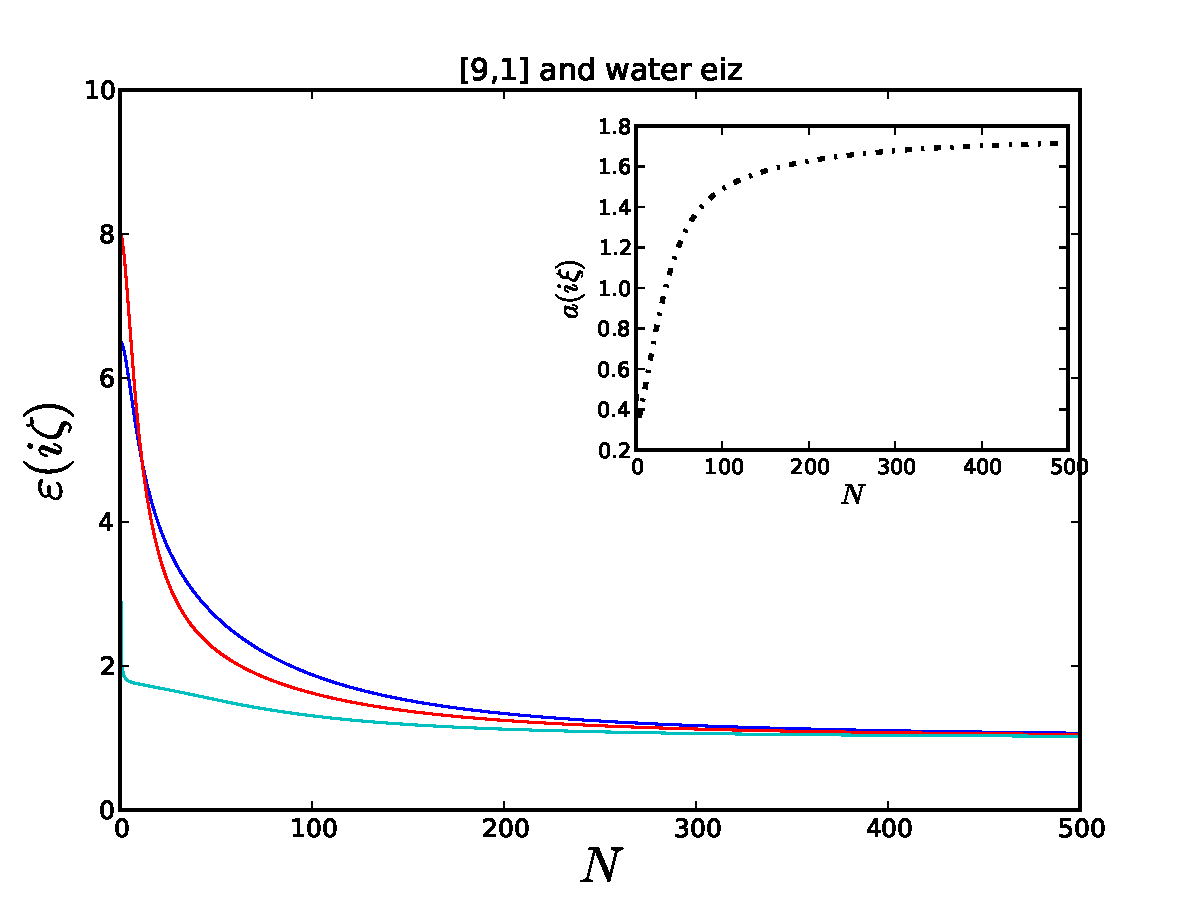
\includegraphics[width=1.0\textwidth]{prop_plots/91w91_eiz.pdf} (b)
\end{center}
\end{minipage}
\caption{Full result using Eqs.\ref{pars-31},\ref{pars-31-g} (a) Anisotropic response functions for CG-10 DNA and water. The DNA response functions in the x and y directions were used as perpendicular and parallel inputs, respectively.  CG-10 and water eps2 data was provided by Dan Dryden. CG-10 data scales Wai-Yim's calculations by 4.94 and is assumed to include Na (more info in Dan Dryden email sent to us on Nov. 8, 2013).  Water data was built from lorentz oscillators R.H.French,J.Amer.Ceram Soc.,83,9,2117-46(2000), H.D.Ackler, et al,J.Coll.Interface Sci.179,46.
(b) Anisotropy metric $a_{1,2}(i\zeta_n)$ using Eq.\ref{eq:adef}, compares the anisotropy of the  cylinders (DNA) to their intervening material, water for the terms contruting to the Matsubara sum.}
\label{eiz91}
\end{center}
\end{figure*} 

%%%%%%%%%EPS2 and Aiz%%%%%%%%%%%%%%%%%%%%%%%%%%%%%%%%%%%%%%%%%%%%%%%%
\begin{figure*}[t!]
\begin{center}
\begin{minipage}[b]{0.40\textwidth}
\begin{center}
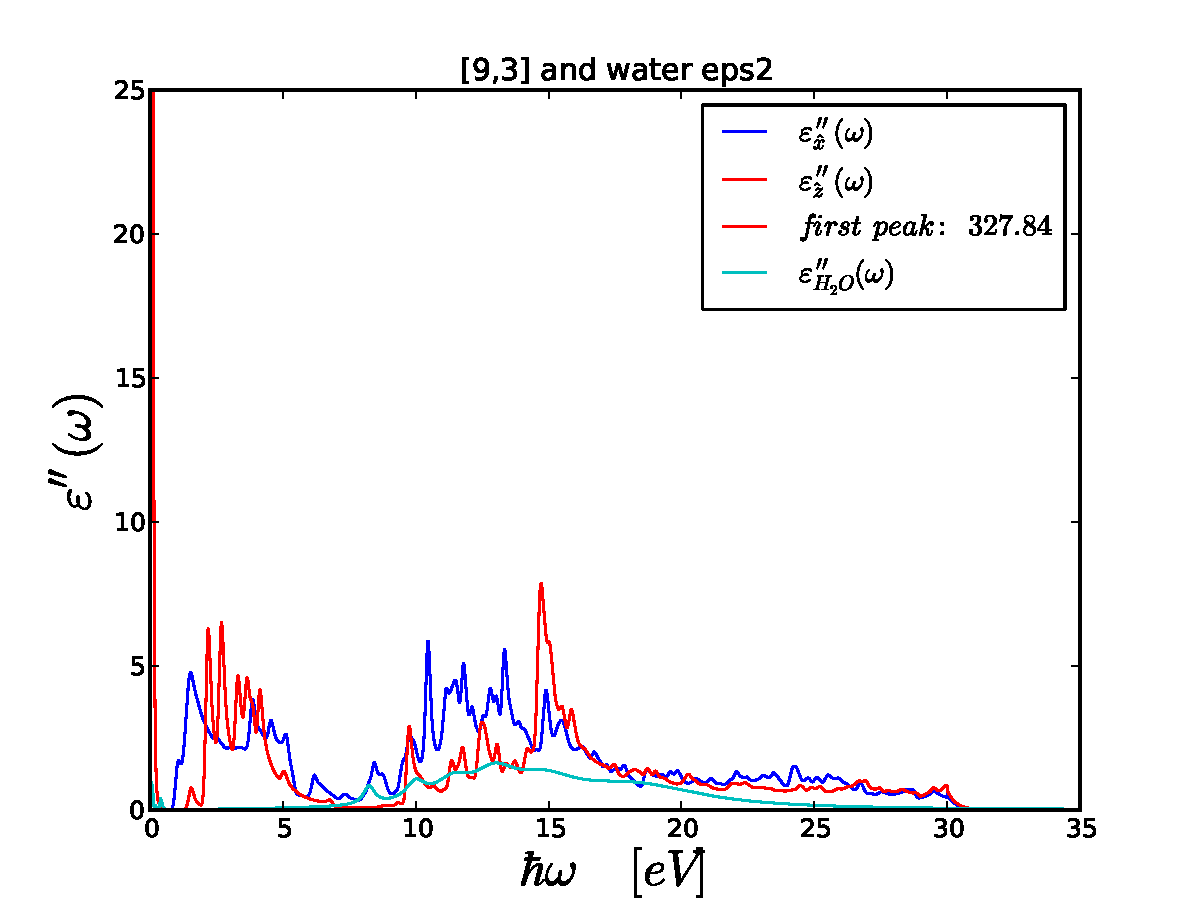
\includegraphics[width=1.0\textwidth]{prop_plots/93w93_eps2.pdf} (a)
\end{center}
\end{minipage}
\hskip 43pt
\begin{minipage}[b]{0.40\textwidth}
\begin{center}
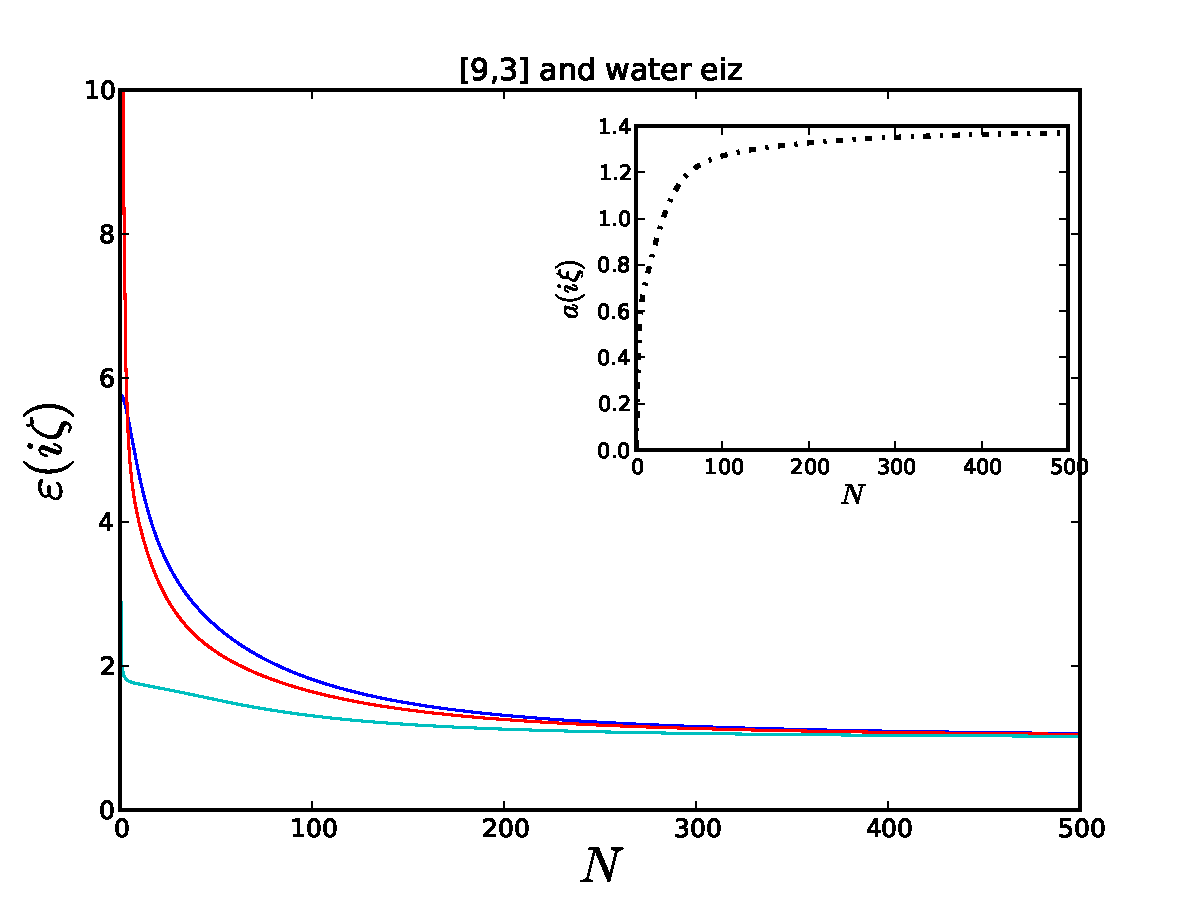
\includegraphics[width=1.0\textwidth]{prop_plots/93w93_eiz.pdf} (b)
\end{center}
\end{minipage}
\caption{Full result using Eqs.\ref{pars-31},\ref{pars-31-g} (a) Anisotropic response functions for CG-10 DNA and water. The DNA response functions in the x and y directions were used as perpendicular and parallel inputs, respectively.  CG-10 and water eps2 data was provided by Dan Dryden. CG-10 data scales Wai-Yim's calculations by 4.94 and is assumed to include Na (more info in Dan Dryden email sent to us on Nov. 8, 2013).  Water data was built from lorentz oscillators R.H.French,J.Amer.Ceram Soc.,83,9,2117-46(2000), H.D.Ackler, et al,J.Coll.Interface Sci.179,46.
(b) Anisotropy metric $a_{1,2}(i\zeta_n)$ using Eq.\ref{eq:adef}, compares the anisotropy of the  cylinders (DNA) to their intervening material, water for the terms contruting to the Matsubara sum.}
\label{eiz93}
\end{center}
\end{figure*} 

%%%%%%%%%EPS2 and Aiz%%%%%%%%%%%%%%%%%%%%%%%%%%%%%%%%%%%%%%%%%%%%%%%%
\begin{figure*}[t!]
\begin{center}
\begin{minipage}[b]{0.40\textwidth}
\begin{center}
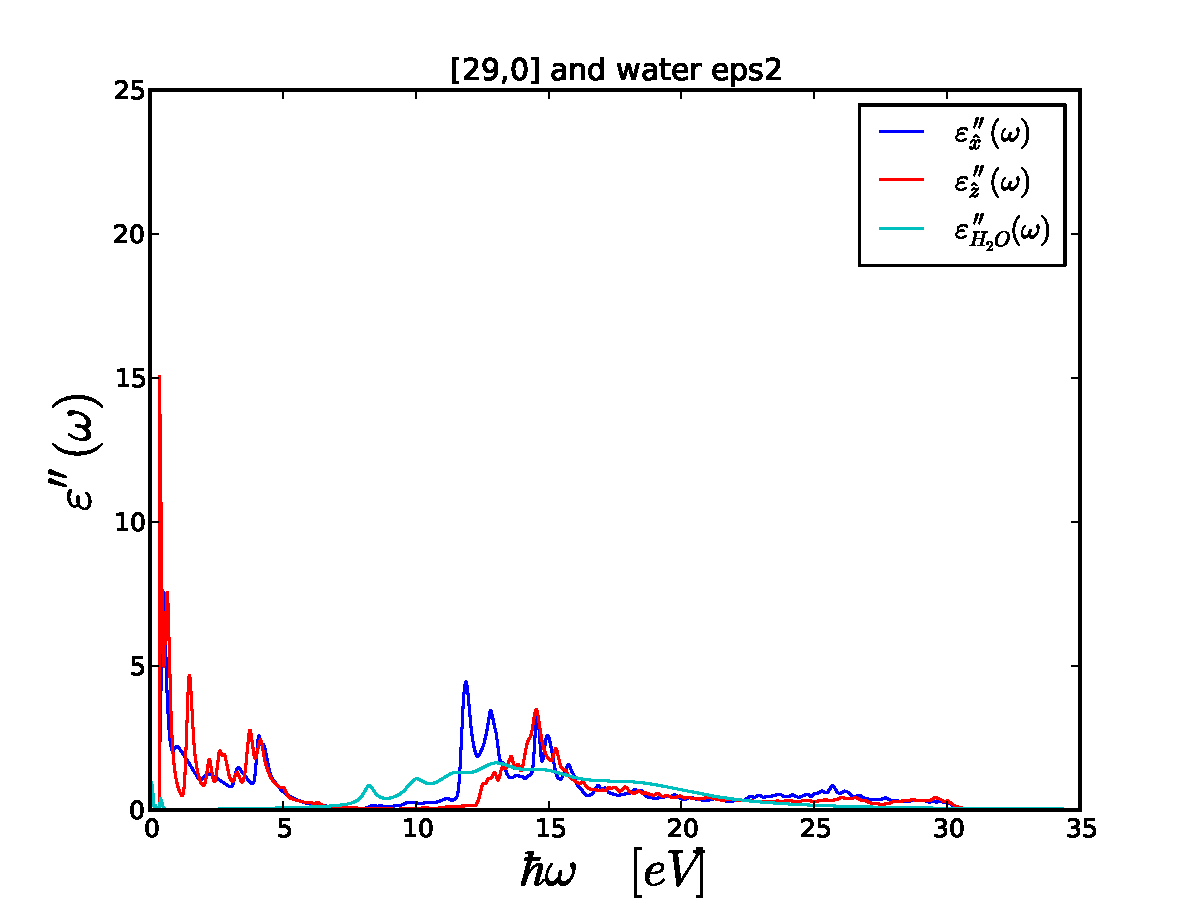
\includegraphics[width=1.0\textwidth]{prop_plots/290w290_eps2.pdf} (a)
\end{center}
\end{minipage}
\hskip 43pt
\begin{minipage}[b]{0.40\textwidth}
\begin{center}
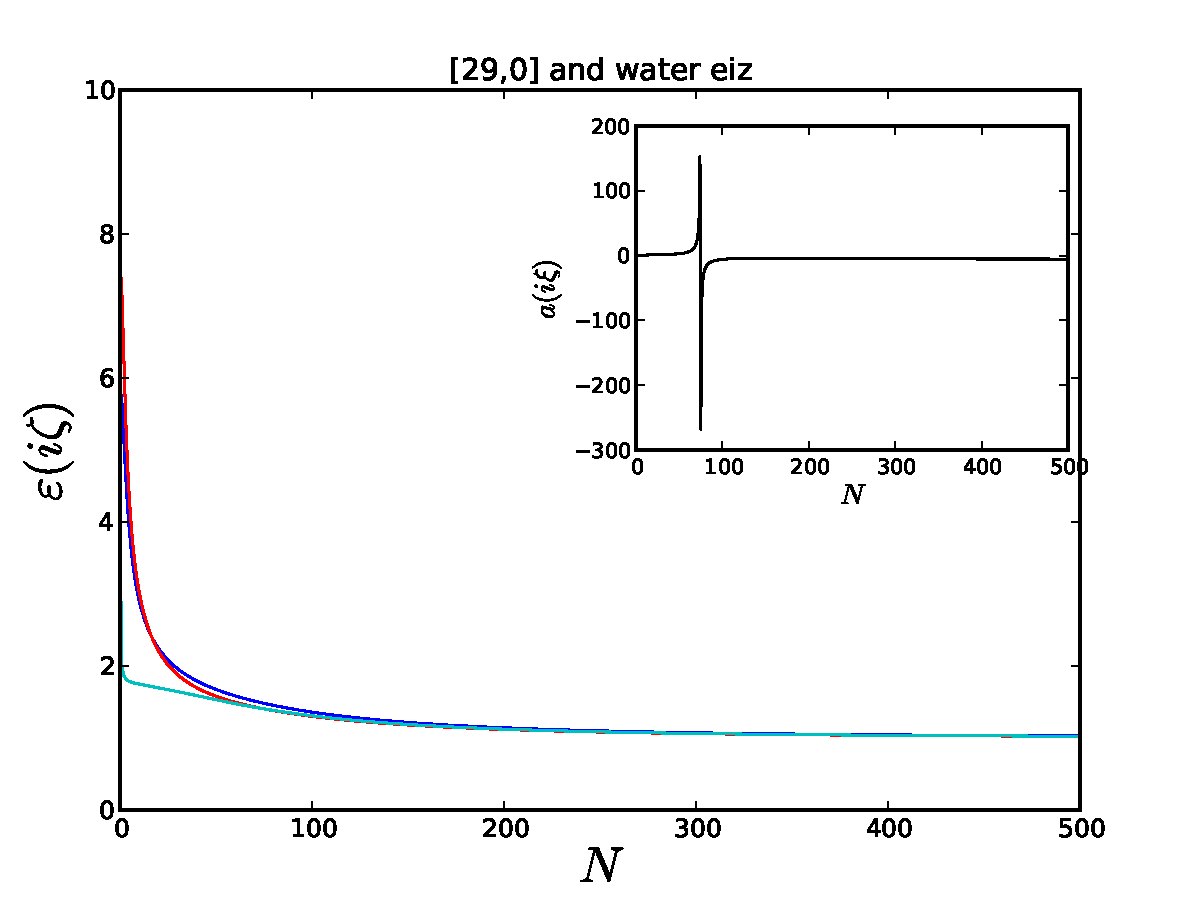
\includegraphics[width=1.0\textwidth]{prop_plots/290w290_eiz.pdf} (b)
\end{center}
\end{minipage}
\caption{Full result using Eqs.\ref{pars-31},\ref{pars-31-g} (a) Anisotropic response functions for CG-10 DNA and water. The DNA response functions in the x and y directions were used as perpendicular and parallel inputs, respectively.  CG-10 and water eps2 data was provided by Dan Dryden. CG-10 data scales Wai-Yim's calculations by 4.94 and is assumed to include Na (more info in Dan Dryden email sent to us on Nov. 8, 2013).  Water data was built from lorentz oscillators R.H.French,J.Amer.Ceram Soc.,83,9,2117-46(2000), H.D.Ackler, et al,J.Coll.Interface Sci.179,46.
(b) Anisotropy metric $a_{1,2}(i\zeta_n)$ using Eq.\ref{eq:adef}, compares the anisotropy of the  cylinders (DNA) to their intervening material, water for the terms contruting to the Matsubara sum.}
\label{eiz290}
\end{center}
\end{figure*} 

%\section{Anisotropy Metric}
%The ratios between the relative anisotropy measures (Eq. \ref{anisoind}) defined as 
%\begin{equation}
%a = \frac{2 \Delta_{\perp}}{\Delta_{\parallel}} = 2 \frac{({\epsilon^{c}}_{\perp}-\epsilon_{m}) \epsilon_{m}}{({\epsilon^{c}}_{\perp}+\epsilon_{m}) ({\epsilon^{c}}_{\parallel}-\epsilon_{m})}
%\label{eq:adef}
%\end{equation}


\begin{figure}
\centerline{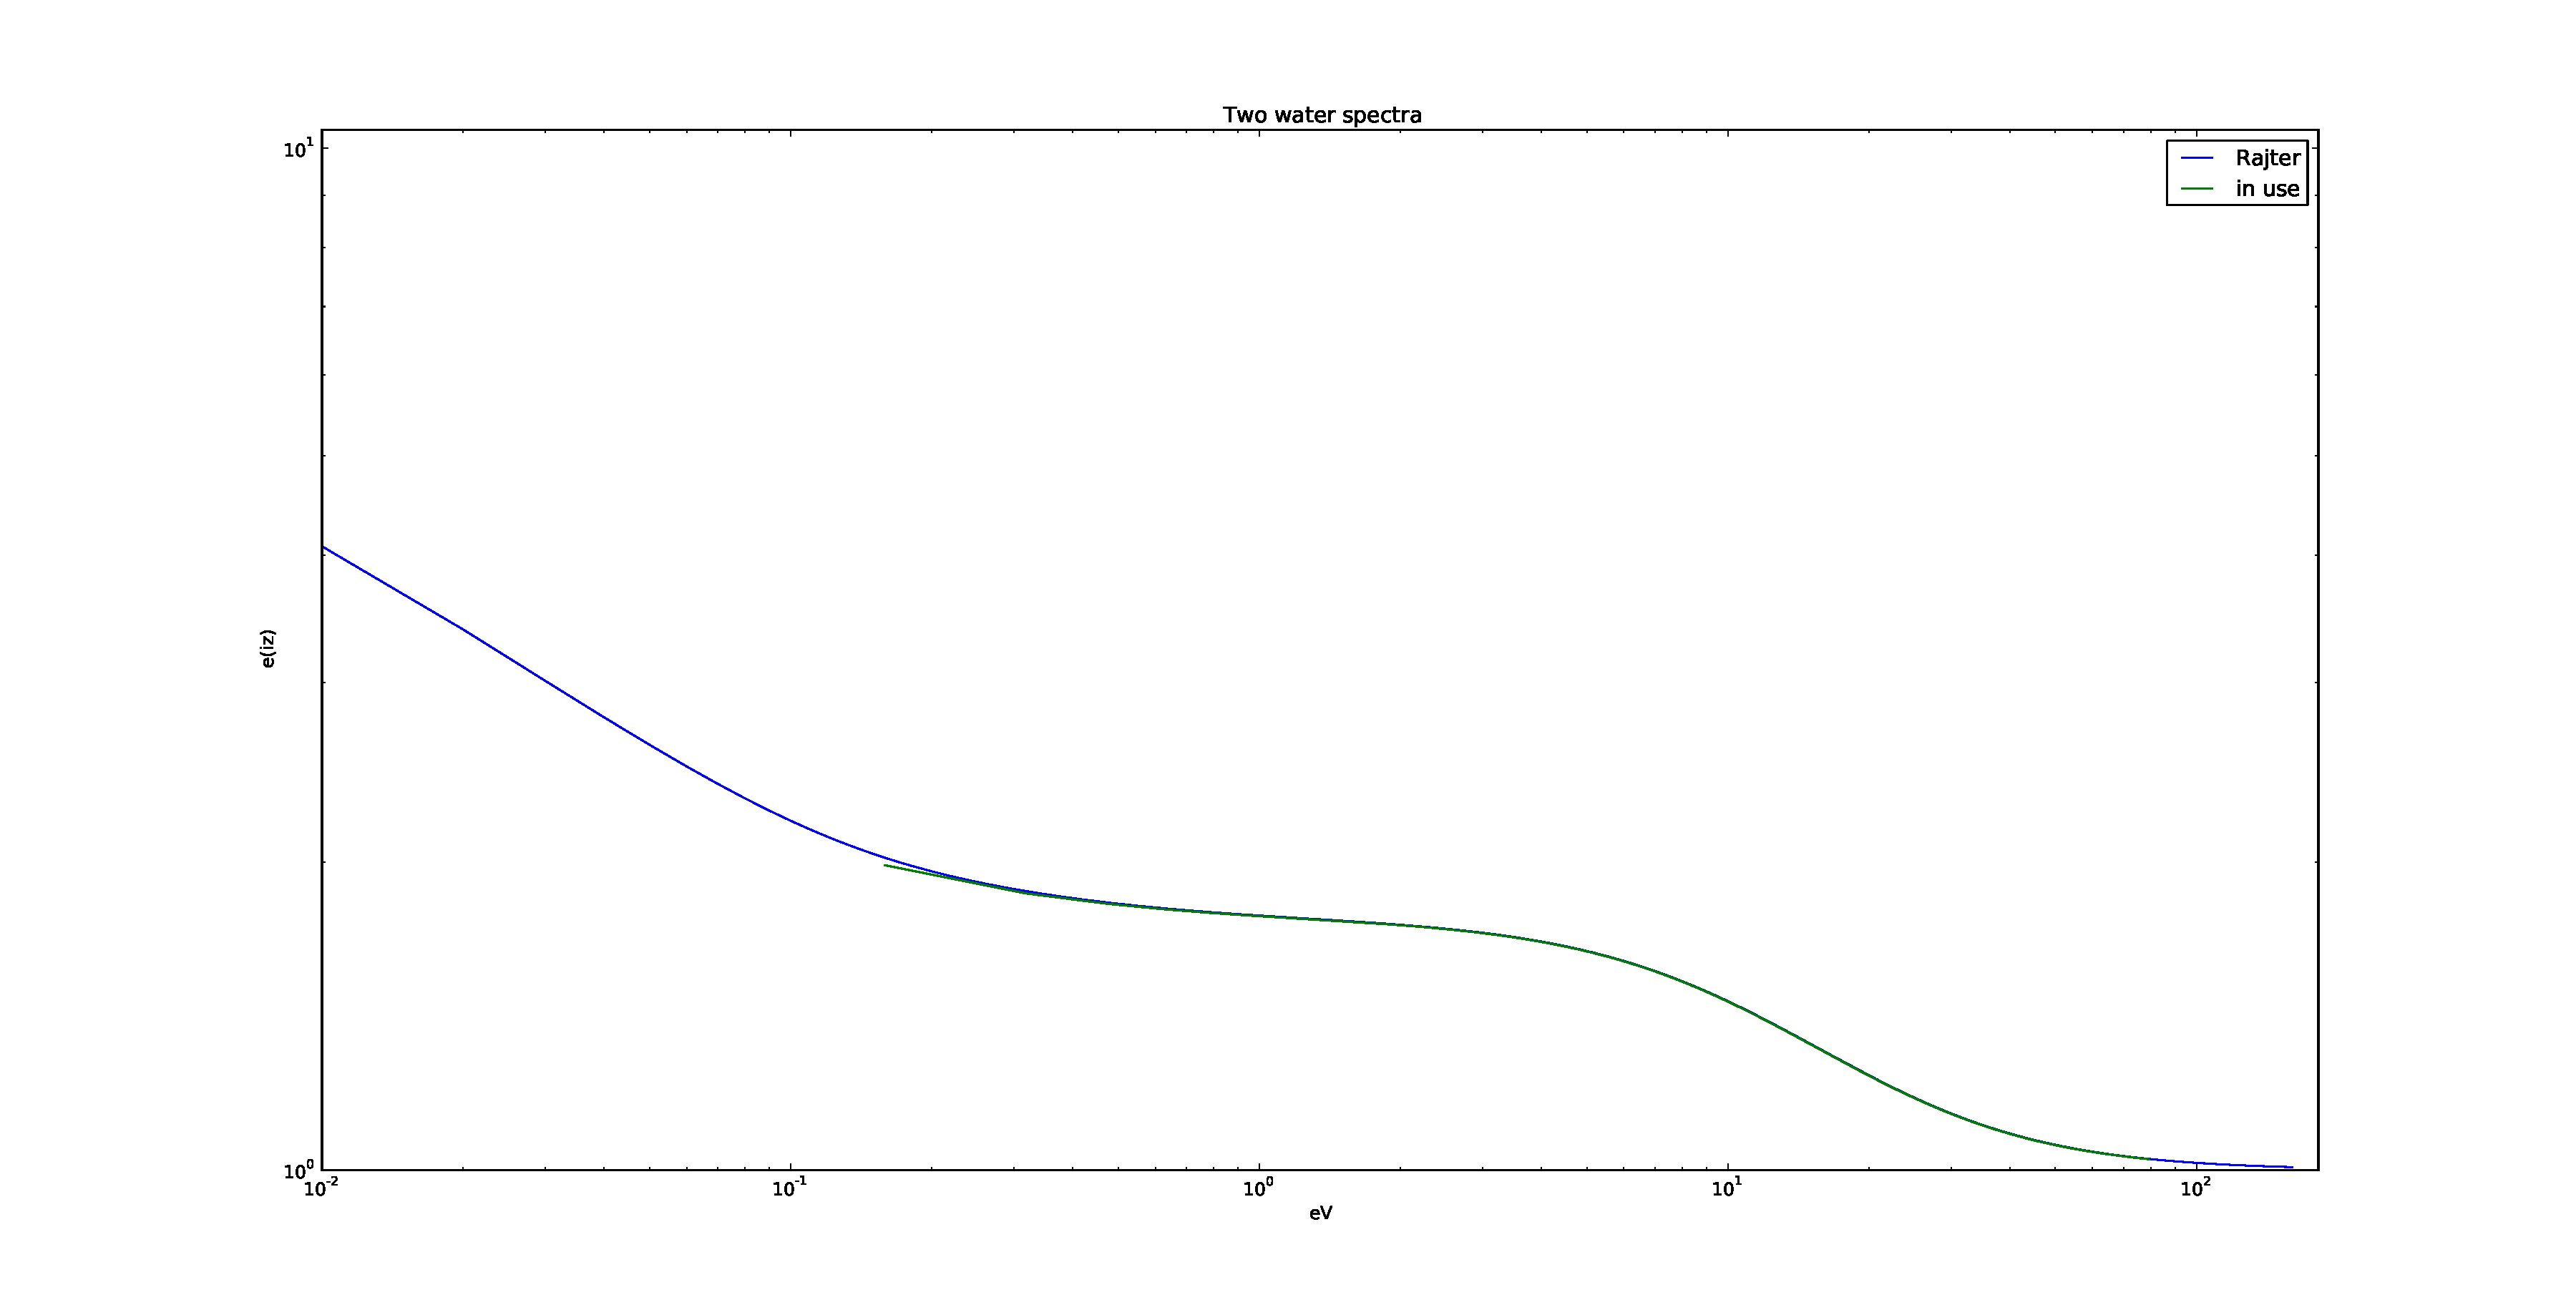
\includegraphics[width=17cm]{two_water_LDS.pdf}}
%\epsfig {file=sketch.pdf,width=5cm}}
\caption{Loglog plot of $\varepsilon(i\xi)$. Ratjer's spectrum (blue) is a
function of continuous energy values and contains a
large peak at n= 0. The current spectrum (green) that is used in Python is the
K-K transform of eps2 data generated by Dan.  Gecko Hamaker also uses Dan's eps2
but may have a different range for its LDS compared to the one plotted in green.}
\label{fig:2xLDS}
\end{figure}
%
%\section{Perpendicular cylinders}
%
%\subsection{Fully retarded}
%
%%%%%%%%%EPS2 and Aiz%%%%%%%%%%%%%%%%%%%%%%%%%%%%%%%%%%%%%%%%%%%%%%%%
\begin{figure*}[t!]
\begin{center}
\begin{minipage}[b]{0.40\textwidth}
\begin{center}
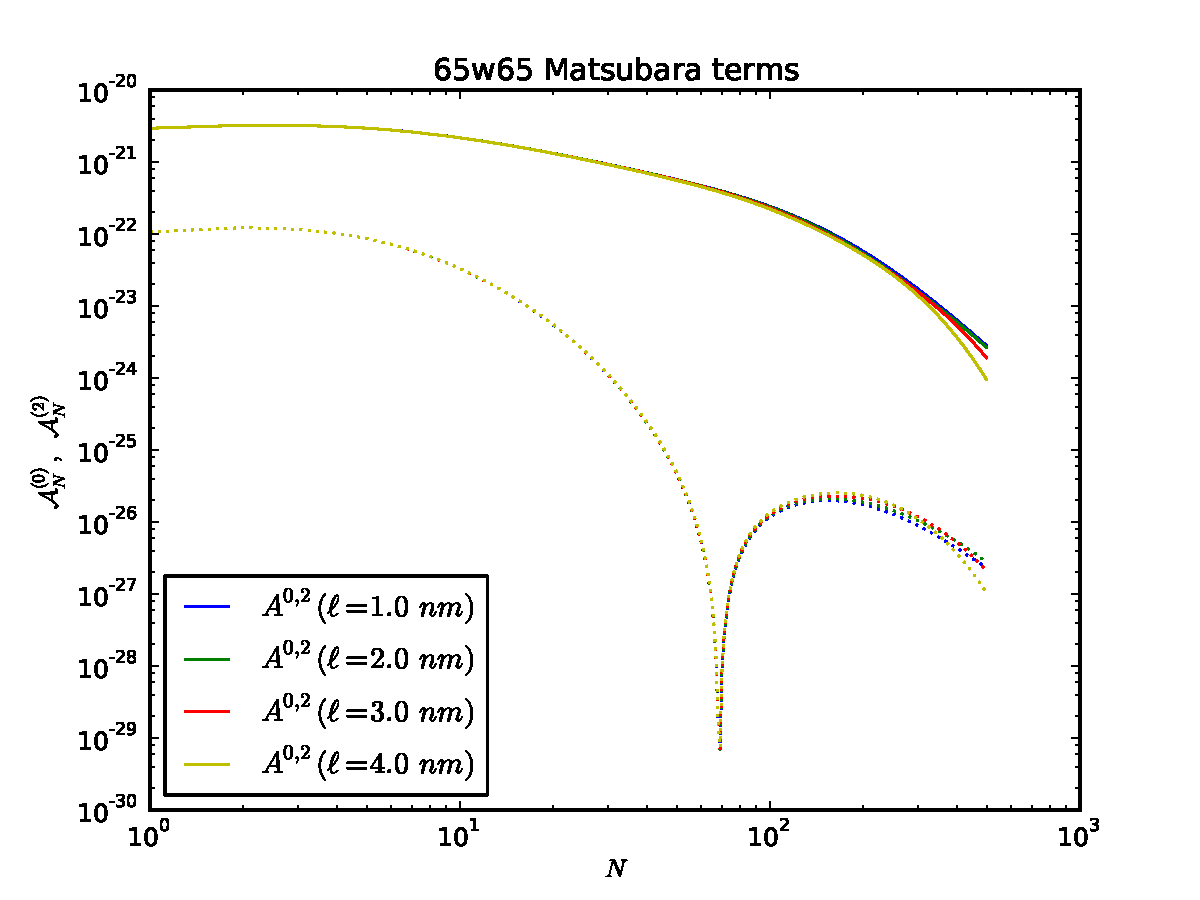
\includegraphics[width=1.2\textwidth]{plots/65_A_vs_n.pdf} (a)
\end{center}
\end{minipage}
\hskip 43pt
\begin{minipage}[b]{0.40\textwidth}
\begin{center}
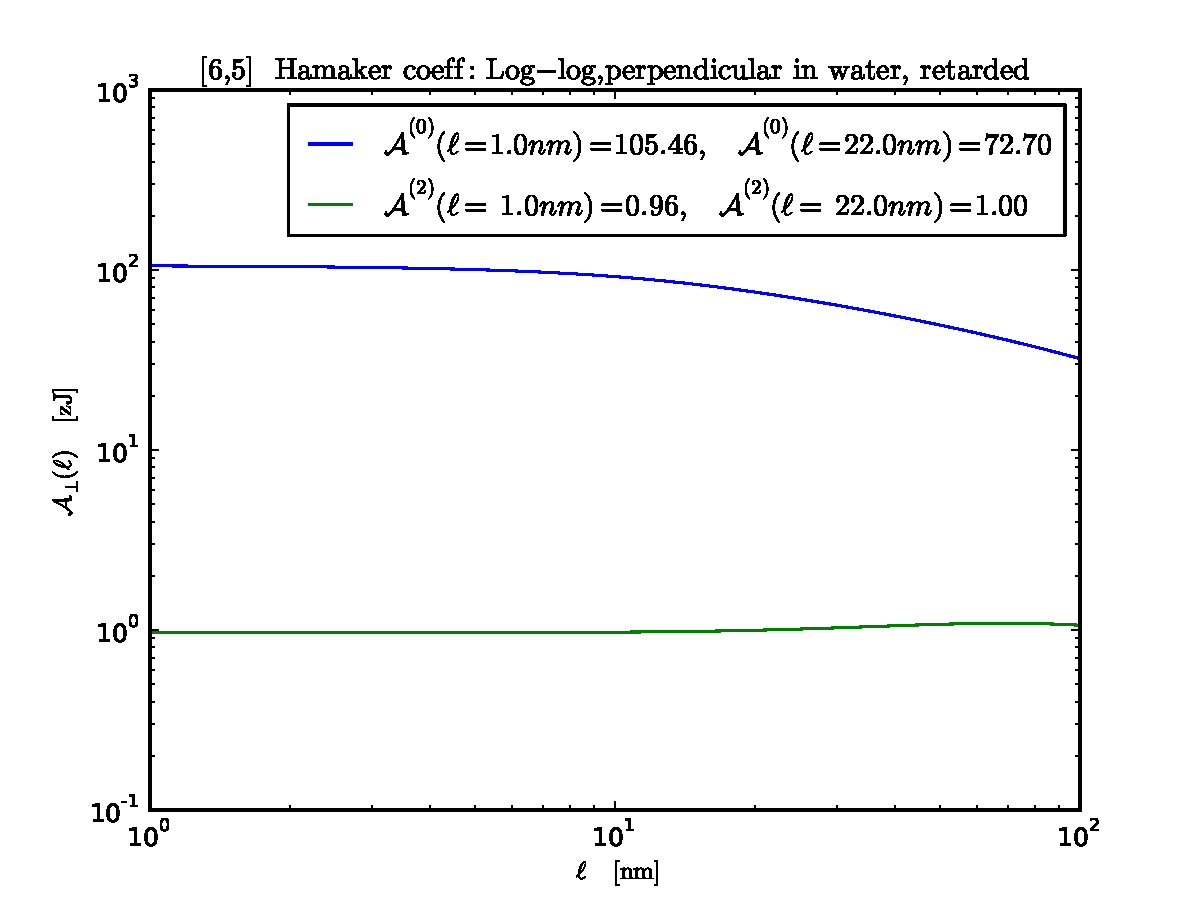
\includegraphics[width=1.2\textwidth]{plots/140322_65w65_HCs_perpendicular_ret.pdf} (b)
\end{center}
\end{minipage}
\caption{Full result using Eqs.\ref{pars-31},\ref{pars-31-g} (a) Anisotropic response functions for CG-10 DNA and water. The DNA response functions in the x and y directions were used as perpendicular and parallel inputs, respectively.  CG-10 and water eps2 data was provided by Dan Dryden. CG-10 data scales Wai-Yim's calculations by 4.94 and is assumed to include Na (more info in Dan Dryden email sent to us on Nov. 8, 2013).  Water data was built from lorentz oscillators R.H.French,J.Amer.Ceram Soc.,83,9,2117-46(2000), H.D.Ackler, et al,J.Coll.Interface Sci.179,46.
(b) Anisotropy metric $a_{1,2}(i\zeta_n)$ using Eq.\ref{eq:adef}, compares the anisotropy of the  cylinders (DNA) to their intervening material, water for the terms contruting to the Matsubara sum.}
\label{eiz65}
\end{center}
\end{figure*} 

%%%%%%%%%EPS2 and Aiz%%%%%%%%%%%%%%%%%%%%%%%%%%%%%%%%%%%%%%%%%%%%%%%%
\begin{figure*}[t!]
\begin{center}
\begin{minipage}[b]{0.40\textwidth}
\begin{center}
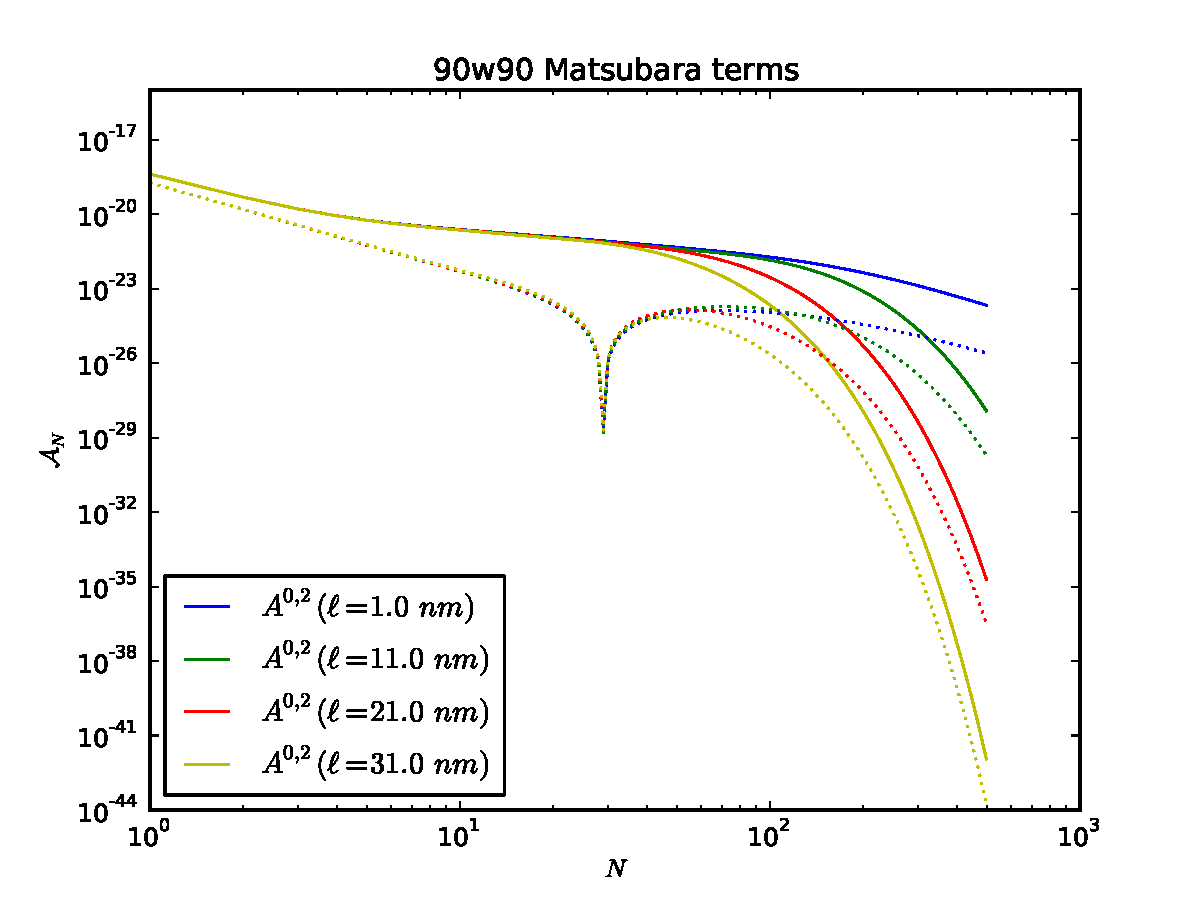
\includegraphics[width=1.2\textwidth]{plots/90_A_vs_n.pdf} (a)
\end{center}
\end{minipage}
\hskip 43pt
\begin{minipage}[b]{0.40\textwidth}
\begin{center}
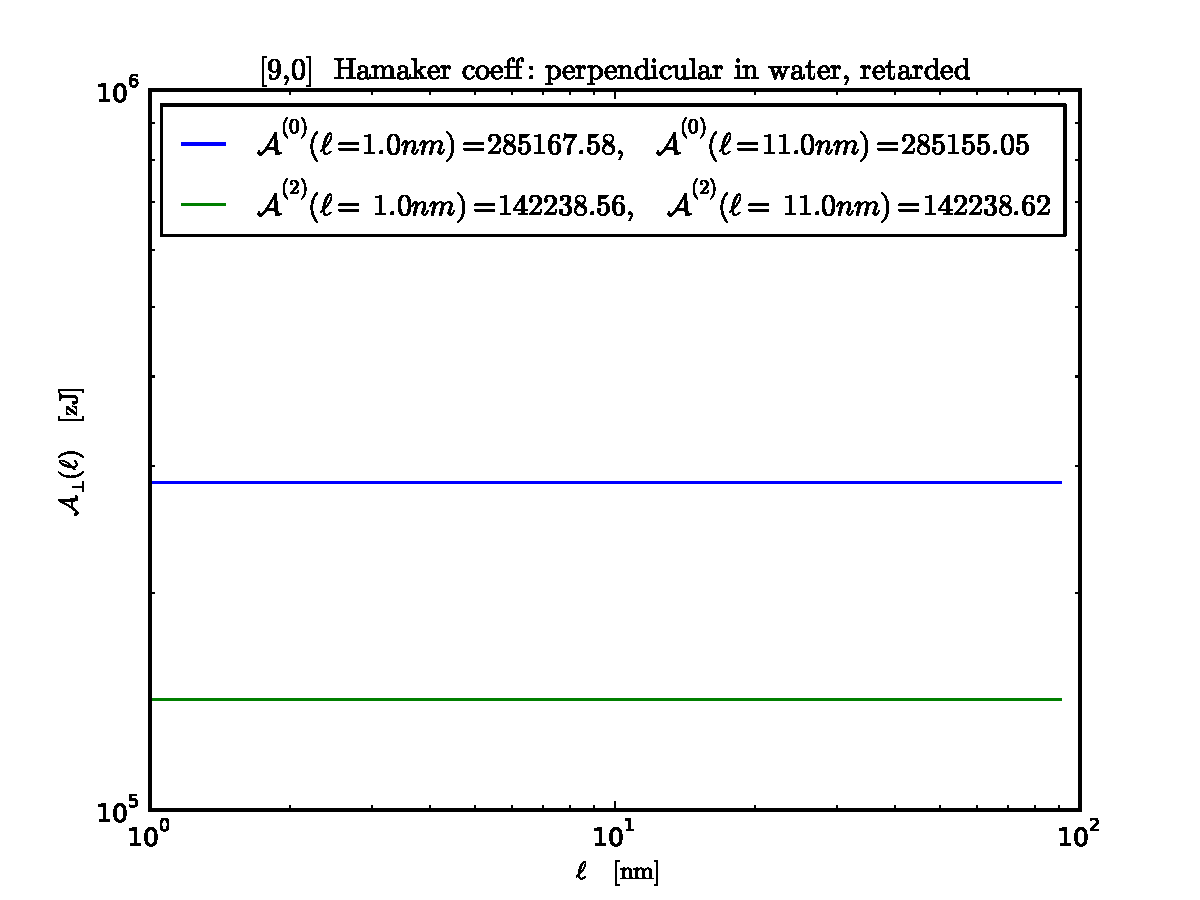
\includegraphics[width=1.2\textwidth]{plots/140322_90w90_HCs_perpendicular_ret.pdf} (b)
\end{center}
\end{minipage}
\caption{Full result using Eqs.\ref{pars-31},\ref{pars-31-g} (a) Anisotropic response functions for CG-10 DNA and water. The DNA response functions in the x and y directions were used as perpendicular and parallel inputs, respectively.  CG-10 and water eps2 data was provided by Dan Dryden. CG-10 data scales Wai-Yim's calculations by 4.94 and is assumed to include Na (more info in Dan Dryden email sent to us on Nov. 8, 2013).  Water data was built from lorentz oscillators R.H.French,J.Amer.Ceram Soc.,83,9,2117-46(2000), H.D.Ackler, et al,J.Coll.Interface Sci.179,46.
(b) Anisotropy metric $a_{1,2}(i\zeta_n)$ using Eq.\ref{eq:adef}, compares the anisotropy of the  cylinders (DNA) to their intervening material, water for the terms contruting to the Matsubara sum.}
\label{eiz65}
\end{center}
\end{figure*} 

%%%%%%%%%EPS2 and Aiz%%%%%%%%%%%%%%%%%%%%%%%%%%%%%%%%%%%%%%%%%%%%%%%%
\begin{figure*}[t!]
\begin{center}
\begin{minipage}[b]{0.40\textwidth}
\begin{center}
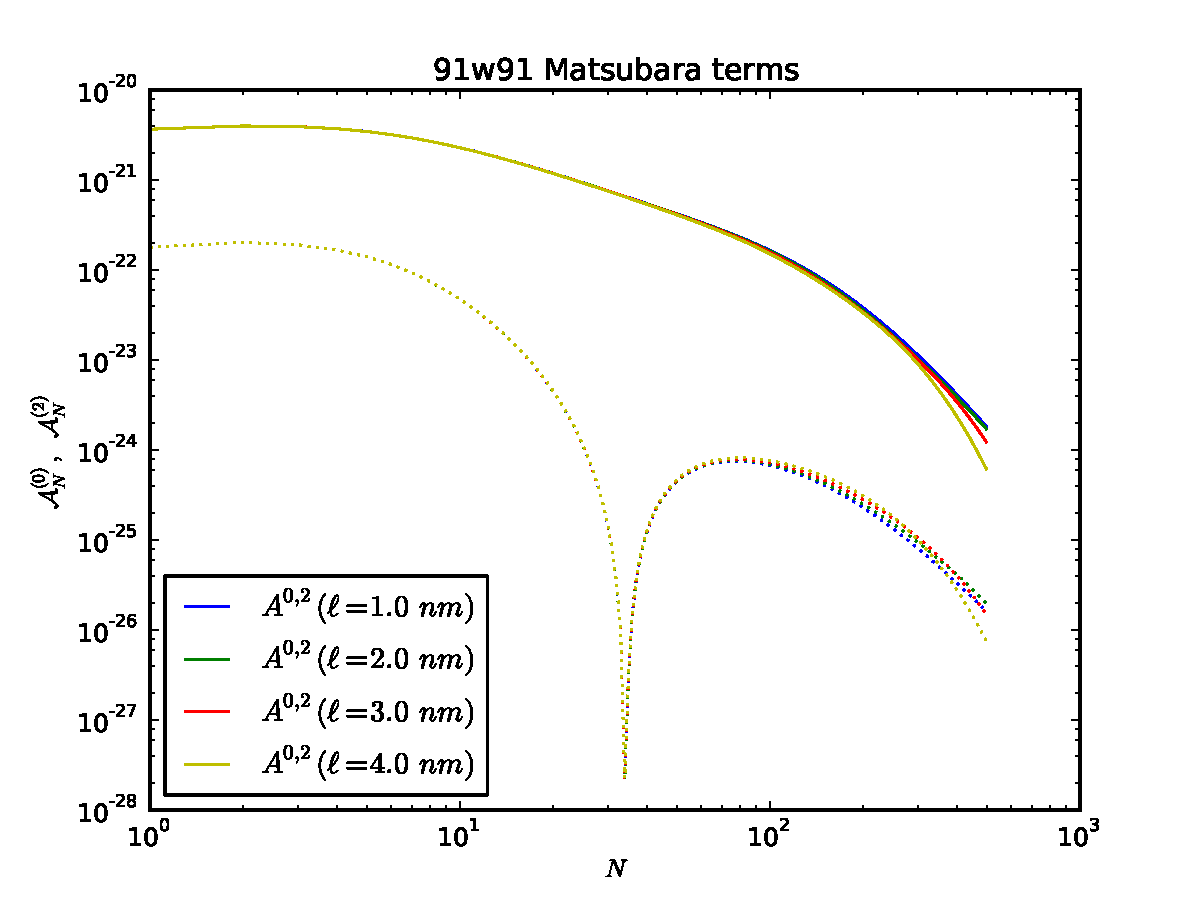
\includegraphics[width=1.2\textwidth]{plots/91_A_vs_n.pdf} (a)
\end{center}
\end{minipage}
\hskip 43pt
\begin{minipage}[b]{0.40\textwidth}
\begin{center}
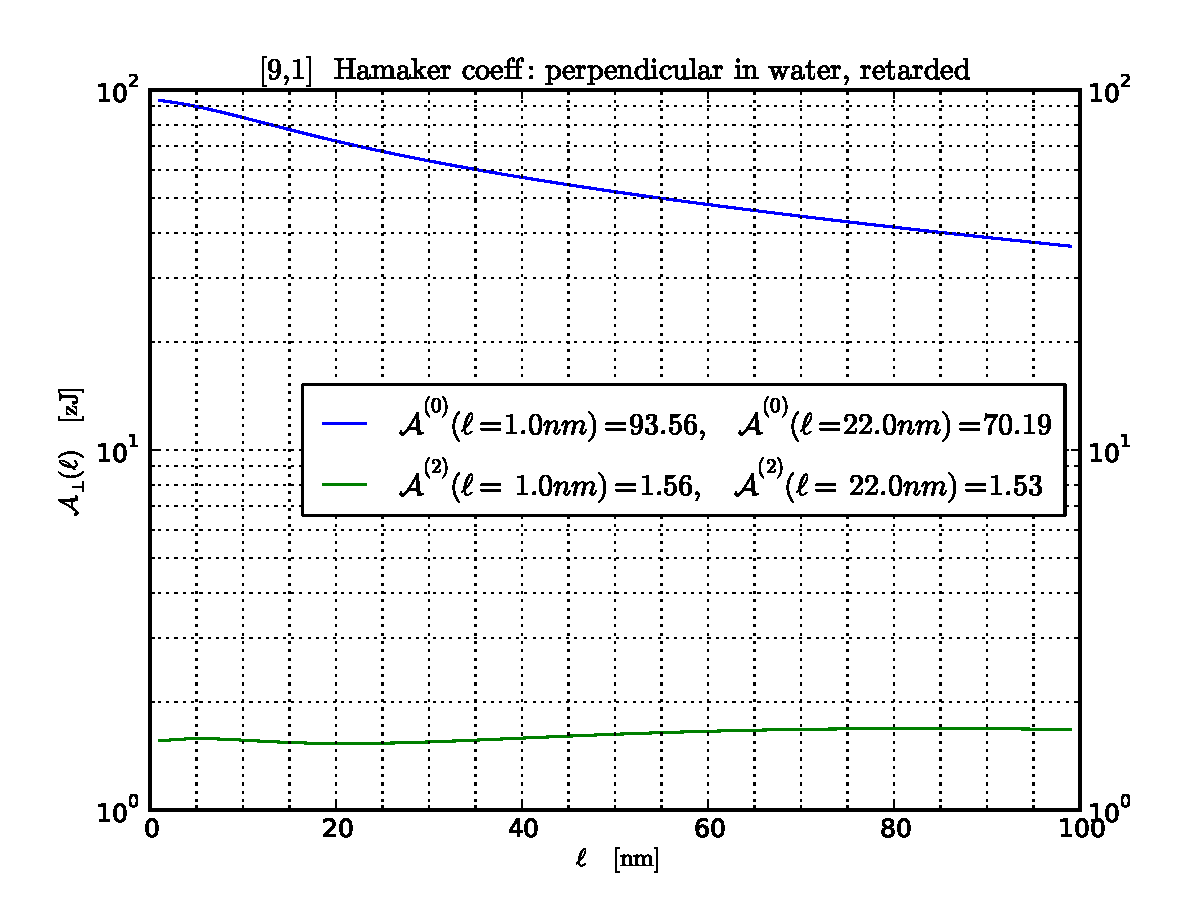
\includegraphics[width=1.2\textwidth]{plots/140322_91w91_HCs_perpendicular_ret.pdf} (b)
\end{center}
\end{minipage}
\caption{Full result using Eqs.\ref{pars-31},\ref{pars-31-g} (a) Anisotropic response functions for CG-10 DNA and water. The DNA response functions in the x and y directions were used as perpendicular and parallel inputs, respectively.  CG-10 and water eps2 data was provided by Dan Dryden. CG-10 data scales Wai-Yim's calculations by 4.94 and is assumed to include Na (more info in Dan Dryden email sent to us on Nov. 8, 2013).  Water data was built from lorentz oscillators R.H.French,J.Amer.Ceram Soc.,83,9,2117-46(2000), H.D.Ackler, et al,J.Coll.Interface Sci.179,46.
(b) Anisotropy metric $a_{1,2}(i\zeta_n)$ using Eq.\ref{eq:adef}, compares the anisotropy of the  cylinders (DNA) to their intervening material, water for the terms contruting to the Matsubara sum.}
\label{eiz65}
\end{center}
\end{figure*} 

%%%%%%%%%EPS2 and Aiz%%%%%%%%%%%%%%%%%%%%%%%%%%%%%%%%%%%%%%%%%%%%%%%%
\begin{figure*}[t!]
\begin{center}
\begin{minipage}[b]{0.40\textwidth}
\begin{center}
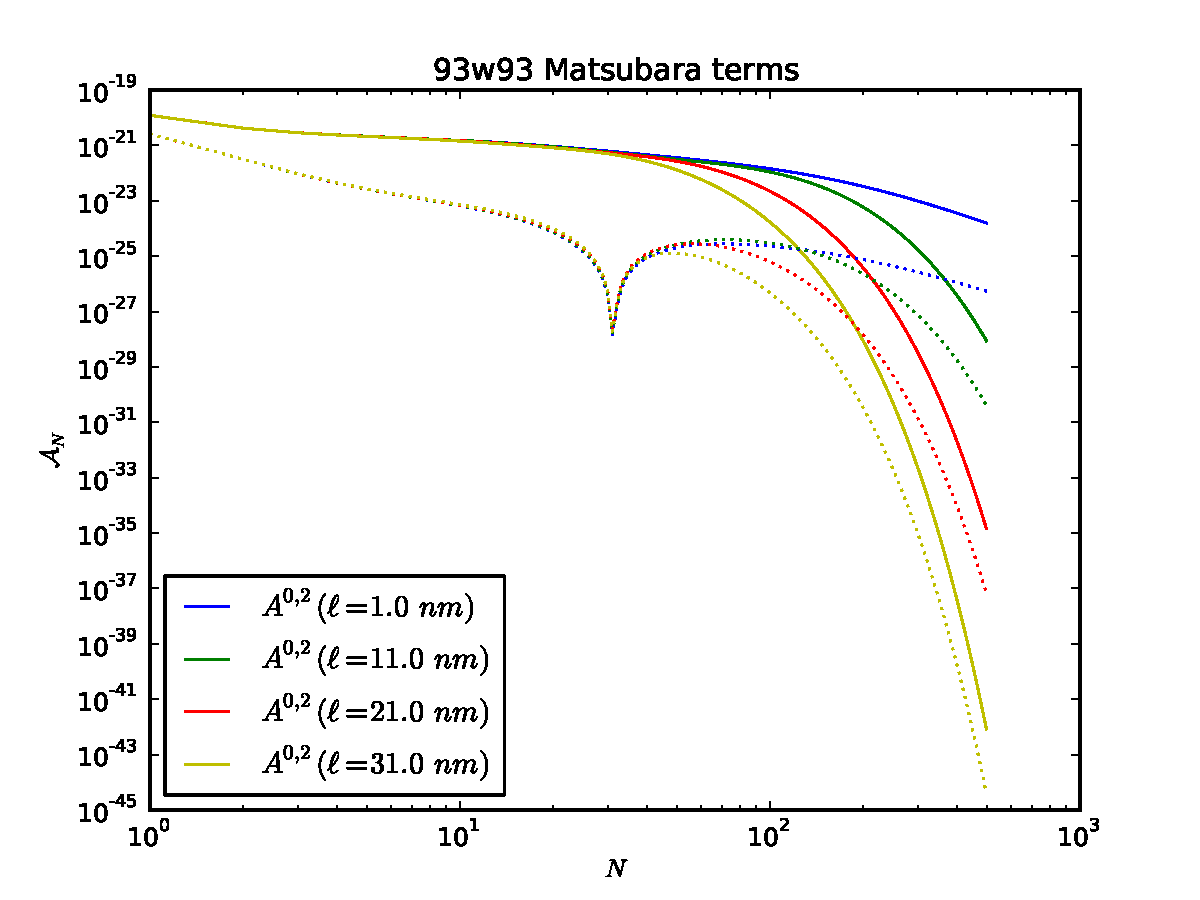
\includegraphics[width=1.2\textwidth]{plots/93_A_vs_n.pdf} (a)
\end{center}
\end{minipage}
\hskip 43pt
\begin{minipage}[b]{0.40\textwidth}
\begin{center}
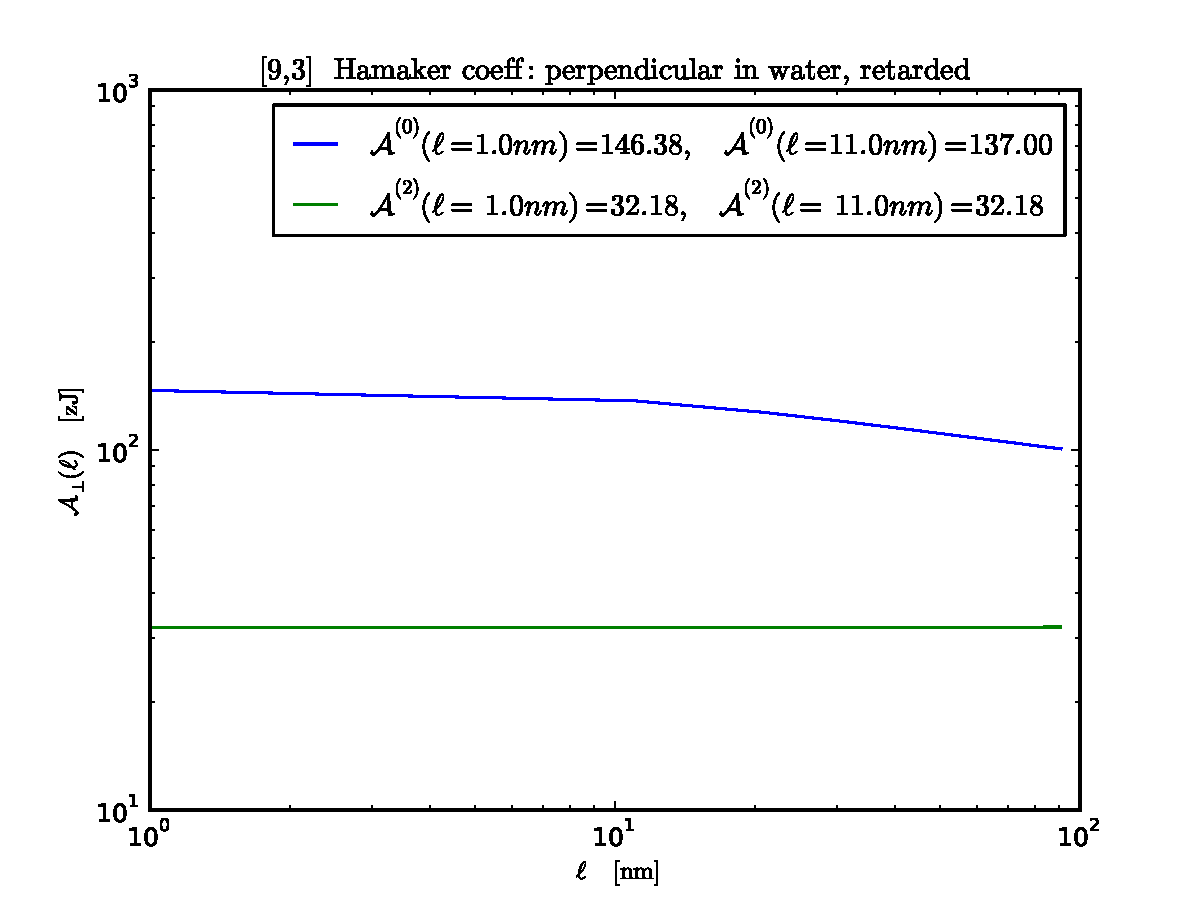
\includegraphics[width=1.2\textwidth]{plots/140322_93w93_HCs_perpendicular_ret.pdf} (b)
\end{center}
\end{minipage}
\caption{Full result using Eqs.\ref{pars-31},\ref{pars-31-g} (a) Anisotropic response functions for CG-10 DNA and water. The DNA response functions in the x and y directions were used as perpendicular and parallel inputs, respectively.  CG-10 and water eps2 data was provided by Dan Dryden. CG-10 data scales Wai-Yim's calculations by 4.94 and is assumed to include Na (more info in Dan Dryden email sent to us on Nov. 8, 2013).  Water data was built from lorentz oscillators R.H.French,J.Amer.Ceram Soc.,83,9,2117-46(2000), H.D.Ackler, et al,J.Coll.Interface Sci.179,46.
(b) Anisotropy metric $a_{1,2}(i\zeta_n)$ using Eq.\ref{eq:adef}, compares the anisotropy of the  cylinders (DNA) to their intervening material, water for the terms contruting to the Matsubara sum.}
\label{eiz65}
\end{center}
\end{figure*} 

%%%%%%%%%EPS2 and Aiz%%%%%%%%%%%%%%%%%%%%%%%%%%%%%%%%%%%%%%%%%%%%%%%%
\begin{figure*}[t!]
\begin{center}
\begin{minipage}[b]{0.40\textwidth}
\begin{center}
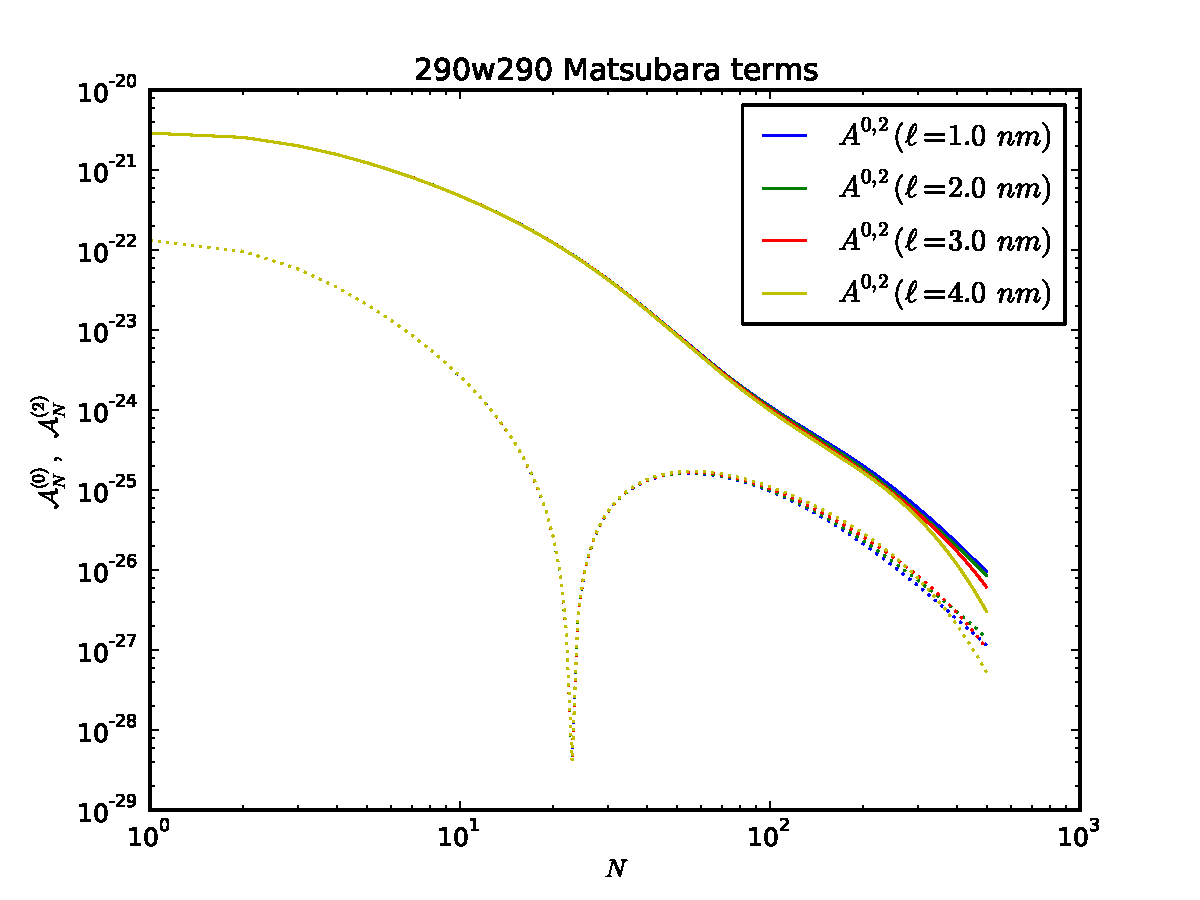
\includegraphics[width=1.2\textwidth]{plots/290_A_vs_n.pdf} (a)
\end{center}
\end{minipage}
\hskip 43pt
\begin{minipage}[b]{0.40\textwidth}
\begin{center}
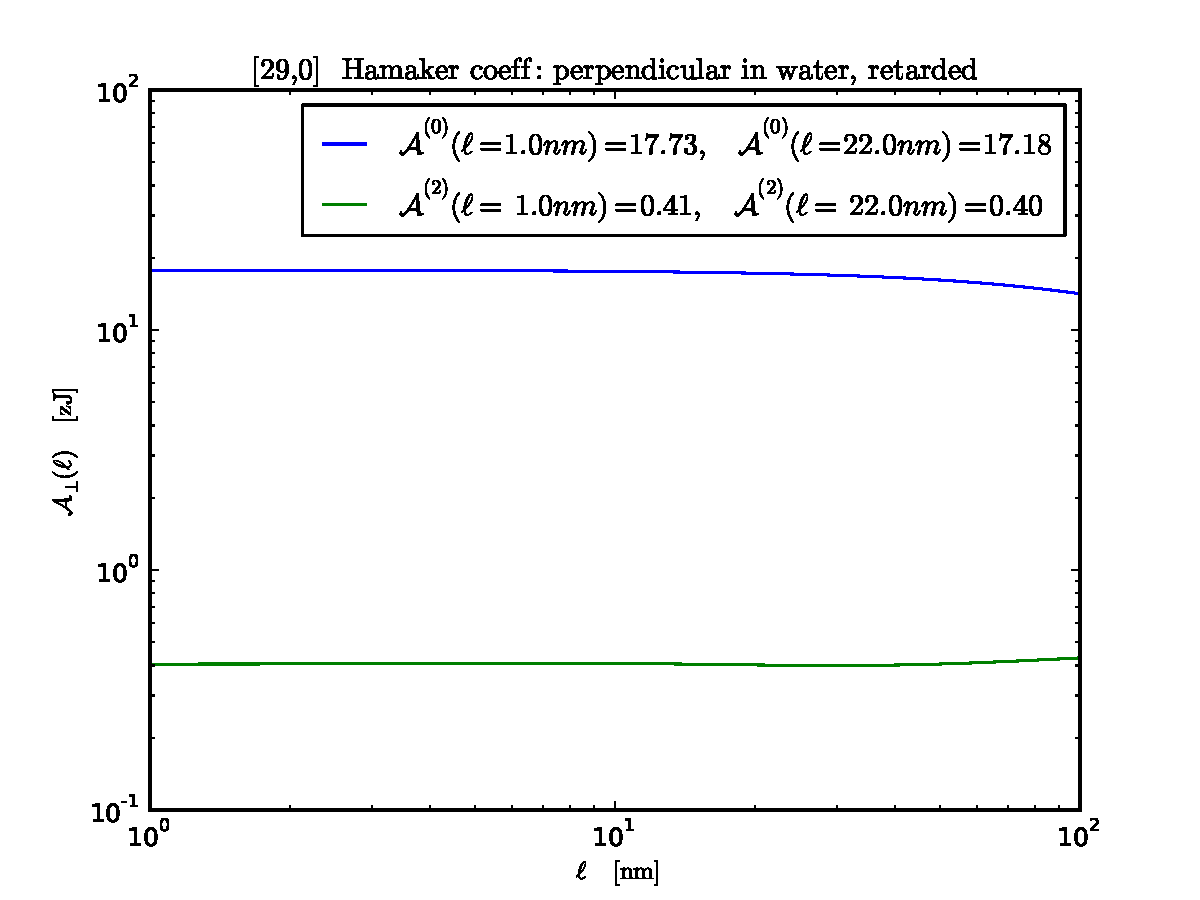
\includegraphics[width=1.2\textwidth]{plots/140322_290w290_HCs_perpendicular_ret.pdf} (b)
\end{center}
\end{minipage}
\caption{Full result using Eqs.\ref{pars-31},\ref{pars-31-g} (a) Anisotropic response functions for CG-10 DNA and water. The DNA response functions in the x and y directions were used as perpendicular and parallel inputs, respectively.  CG-10 and water eps2 data was provided by Dan Dryden. CG-10 data scales Wai-Yim's calculations by 4.94 and is assumed to include Na (more info in Dan Dryden email sent to us on Nov. 8, 2013).  Water data was built from lorentz oscillators R.H.French,J.Amer.Ceram Soc.,83,9,2117-46(2000), H.D.Ackler, et al,J.Coll.Interface Sci.179,46.
(b) Anisotropy metric $a_{1,2}(i\zeta_n)$ using Eq.\ref{eq:adef}, compares the anisotropy of the  cylinders (DNA) to their intervening material, water for the terms contruting to the Matsubara sum.}
\label{eiz65}
\end{center}
\end{figure*} 
\section{Results}

\begin{table}[ht]
\caption{Rajter results from IJMR perpendiuclar cylinders in water (Rajter's
spectrum)}
\centering
\begin{tabular}{l c|c|c}
  \hline  
  &\hspace{0.25in}CNT \hspace{0.25in}& \hspace{0.25in}$\mathcal{A}^{0}$    [zJ] \hspace{0.25in}& \hspace{0.25in}$\mathcal{A}^{2}$    [zJ] \hspace{0.25in}\\
  \hline\hline 
  &[6,5]  & 106 & 1.9 \\
  \hline
  &[9,0]  & \multicolumn{2}{c}{-}\\
  \hline
  &[9,1]  & 92.8 & 3 \\
  \hline
  &[9,3]  & 107 & 36.2 \\
  \hline
  &[29,0] & 18.5 & 0.8 \\
  \hline  
\end{tabular}
\label{table:nonlin}
\end{table}

\begin{table}[ht]
\caption{Gecko Hamaker results from 2.07, perpendiuclar cylinders in water}
\centering
\begin{tabular}{l c|c|c}
  \hline  
  &\hspace{0.25in}CNT \hspace{0.25in}& \hspace{0.25in}$\mathcal{A}^{0}$    [zJ] \hspace{0.25in}& \hspace{0.25in}$\mathcal{A}^{2}$    [zJ] \hspace{0.25in}\\
  \hline\hline 
  &[6,5]  & 100 & 1.04 \\
  \hline
  &[9,0]  & 151 & 6.96 \\
  \hline
  &[9,1]  & 84.85 & 1.16 \\
  \hline
  &[9,3]  & 80.66 & 1.55 \\
  \hline
  &[29,0] & 17.68 & 0.22 \\
  \hline  
\end{tabular}
\label{table:nonlin}
\end{table}

\begin{table}[ht]
\caption{Python results, retarded formulation: perpendiuclar cylinders in water, intersurface distance = 1 nm}
\centering
\begin{tabular}{l c|c|c}
  \hline  
  &\hspace{0.25in}CNT \hspace{0.25in}& \hspace{0.25in}$\mathcal{A}^{0}$    [zJ] \hspace{0.25in}& \hspace{0.25in}$\mathcal{A}^{2}$    [zJ] \hspace{0.25in}\\
  \hline\hline 
  &[6,5]  & 105.46 & 0.96 \\
  \hline
  &[9,0]  & \multicolumn{2}{c}{semi-metal; in progress}\\
  \hline
  &[9,1]  & 93.56 & 1.56 \\
  \hline
  &[9,0]  & \multicolumn{2}{c}{semi-metal; in progress}\\
  \hline
  &[29,0] & 17.73 & 0.41 \\
  \hline  
\end{tabular}
\label{table:nonlin}
\end{table}

\begin{table}[ht]
\caption{Python results, non-retarded formulation: perpendiuclar cylinders in water}% title of Table
\centering
\begin{tabular}{r c | c | c}
  \hline
  &\hspace{0.25in}CNT \hspace{0.25in}& \hspace{0.25in}$\mathcal{A}^{0}$    [zJ] \hspace{0.25in}& \hspace{0.25in}$\mathcal{A}^{2}$    [zJ] \hspace{0.25in}\\
  \hline\hline                       
  &[6,5]  & 126.80 & 1.16 \\
  \hline
  &[9,0]  & \multicolumn{2}{c}{semi-metal; in progress}\\
  \hline
  &[9,1]  & 112.22 & 1.87 \\
  \hline
  &[9,3]  & \multicolumn{2}{c}{semi-metal; in progress}\\
  \hline
  &[29,0] & 20.93 & 0.49 \\
  \hline  
\end{tabular}
\label{table:nonlin}
\end{table}



\end{document}


